\documentclass[11pt]{article}
\usepackage[margin=0.72in]{geometry}
\usepackage{amsmath,amssymb,bm}
\usepackage{booktabs,longtable,array,tabularx,multirow}
\usepackage{graphicx}
\usepackage[dvipsnames,table]{xcolor}
\usepackage{tikz}
\usetikzlibrary{arrows.meta,positioning,fit,calc,shapes.geometric}
\usepackage{hyperref}
\usepackage{caption,subcaption}
\usepackage{enumitem}
\usepackage{fancyhdr}
\usepackage{float}
\usepackage{pdflscape}
\usepackage{microtype}

\hypersetup{colorlinks=true,linkcolor=NavyBlue,urlcolor=RoyalBlue,citecolor=NavyBlue}
\pagestyle{fancy}
\fancyhf{}
\lhead{RGB Self-Recovery Experimental Report}
\rhead{\thepage}
\setlength{\headheight}{14pt}
\setlength{\parindent}{0pt}
\setlength{\parskip}{5pt}
\setlist{nosep,leftmargin=1.5em}

\definecolor{gpred}{HTML}{D73027}
\definecolor{rgbblue}{HTML}{4575B4}
\definecolor{dinoteal}{HTML}{1B9E77}
\definecolor{grupurple}{HTML}{7570B3}
\definecolor{kalmanorange}{HTML}{E08214}
\definecolor{graphgreen}{HTML}{4D9221}
\definecolor{gtsamcyan}{HTML}{00A6A6}
\definecolor{softgray}{HTML}{F2F3F5}

\newcommand{\best}[1]{\textbf{#1}}
\newcommand{\unitm}{\,\mathrm{m}}
\newcommand{\unitdeg}{^{\circ}}
\newcommand{\todoresult}{\colorbox{Yellow!35}{\textbf{IN PROGRESS}}}
\newcommand{\modelbox}[4][]{\node[draw=#2,fill=#2!10,rounded corners,
  minimum width=37mm,minimum height=9mm,align=center,#1] (#3) {#4};}

\title{\textbf{From Frame-Local RGB Recovery to Sequence-Wide Pose Optimization}\\
\large A Reproducible Experimental Report for GigaPose Refinement}
\author{GigaPose / RGB Self-Recovery Development Log}
\date{Results snapshot: 6 August 2026}

\begin{document}
\maketitle

\begin{abstract}
This report consolidates the complete sequence of experiments performed to improve per-frame GigaPose predictions for a single racecar.  The progression starts with an RGB/mask/CAD verifier, extends its visual encoder with frozen DINOv2 and spatial matching U-Nets, introduces a causal GRU candidate selector and a learned GRU--Kalman filter, adds fixed-lag orientation and translation repair, replaces the recurrent cascade with numeric and frozen-visual transformers, and finally performs complete-sequence optimization with a SciPy factor graph and GTSAM.  All reported final tables use the regenerated-pose Assetto Corsa benchmark with 5,174 frames unless explicitly marked as development/validation results.  The best completed balanced system is currently the \emph{translation cascade used as a prior to the SciPy factor graph}, with translation mean/RMSE $2.240/3.674\unitm$, rotation mean/RMSE $11.45/29.76\unitdeg$, and ADD mean/RMSE $2.276/3.695\unitm$.  Using the frozen visual transformer as the SciPy prior produces the best rotation result ($9.26/24.68\unitdeg$ mean/RMSE) and the best translation from 20--80 m, but the translation-cascade prior remains substantially more robust beyond 100 m.
\end{abstract}

\tableofcontents
\newpage

\section{Scope, chronology, and experimental question}

The central question is not whether a temporal model can reproduce a tracking label.  It is:
\begin{quote}
Can RGB appearance, a target instance mask, CAD evidence, and sequence structure correct wrong GigaPose 6D poses---including depth errors and front/rear ambiguity---rather than merely smooth them?
\end{quote}

The implemented progression is summarized in Fig.~\ref{fig:evolution}.  Every major stage remained available as an independent package so that improvements could be attributed to a specific design change.

\begin{figure}[H]
\centering
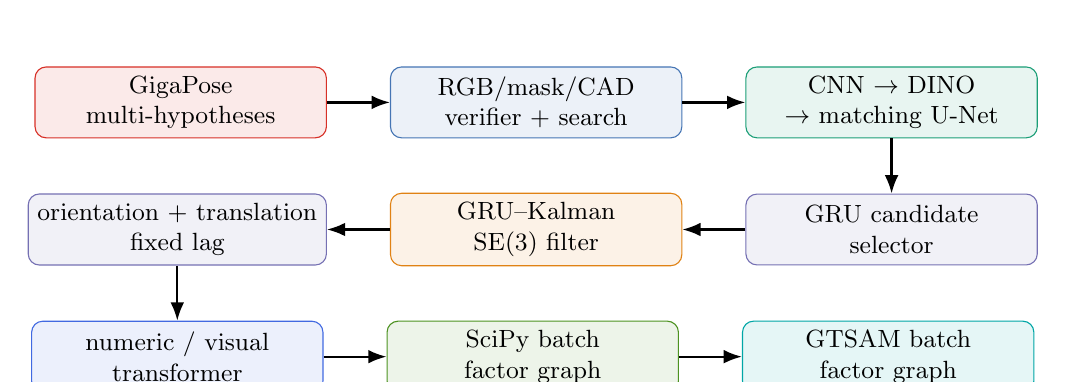
\begin{tikzpicture}[node distance=7mm and 8mm,>=Latex,font=\small]
\modelbox{gpred}{gp}{GigaPose\\multi-hypotheses}
\modelbox[right=of gp]{rgbblue}{rgb}{RGB/mask/CAD\\verifier + search}
\modelbox[right=of rgb]{dinoteal}{visual}{CNN $\rightarrow$ DINO\\$\rightarrow$ matching U-Net}
\modelbox[below=of visual]{grupurple}{gru}{GRU candidate\\selector}
\modelbox[left=of gru]{kalmanorange}{kf}{GRU--Kalman\\SE(3) filter}
\modelbox[left=of kf]{grupurple}{lag}{orientation + translation\\fixed lag}
\modelbox[below=of lag]{RoyalBlue}{tr}{numeric / visual\\transformer}
\modelbox[right=of tr]{graphgreen}{fg}{SciPy batch\\factor graph}
\modelbox[right=of fg]{gtsamcyan}{gs}{GTSAM batch\\factor graph}
\draw[->,thick] (gp.east)--(rgb.west);
\draw[->,thick] (rgb.east)--(visual.west);
\draw[->,thick] (visual.south)--(gru.north);
\draw[->,thick] (gru.west)--(kf.east);
\draw[->,thick] (kf.west)--(lag.east);
\draw[->,thick] (lag.south)--(tr.north);
\draw[->,thick] (tr.east)--(fg.west);
\draw[->,thick] (fg.east)--(gs.west);
\end{tikzpicture}
\caption{Chronological evolution of the pose-refinement work.  Arrows denote the development sequence, not a requirement that every deployed system contain every preceding block.}
\label{fig:evolution}
\end{figure}

\subsection{Benchmark and an important split caveat}

The regenerated benchmark contains 5,174 frames, four physical run names, 3,350 front-camera frames, 1,824 rear-camera frames, and 68 contiguous temporal segments.  The distance-bin counts are shown below.

\begin{center}
\begin{tabular}{lrrrrrrr}
\toprule
Distance (m) & 0--20 & 20--40 & 40--60 & 60--80 & 80--100 & 100--120 & 120--140\\
\midrule
Frames & 862 & 1,854 & 715 & 485 & 568 & 410 & 280\\
\bottomrule
\end{tabular}
\end{center}

Training contains 9,795 frames and validation contains 2,000 frames, with no training/validation or training/benchmark frame overlap.  However, an audit of \texttt{sequence\_run}, camera, and source-frame keys found
\[
|\mathcal V\cap\mathcal T_{\rm benchmark}|=2000.
\]
Thus all numbers in this document are valid reproducible \emph{development-benchmark} measurements, but transformer model-selection and early-stopping decisions have seen the two validation runs that are included in the 5,174-frame benchmark.  A new physical run is required before claiming fully untouched generalization.

\subsection{Metrics}

For ground-truth pose $T^*=[R^*,\bm t^*]$ and prediction $\hat T=[\hat R,\hat{\bm t}]$, translation error is
\begin{equation}
e_t=\|\hat{\bm t}-\bm t^*\|_2.
\end{equation}
Rotation error is the geodesic SO(3) angle
\begin{equation}
e_R=\left\|\log\!\left((R^*)^T\hat R\right)\right\|_2\frac{180}{\pi}.
\end{equation}
For mesh vertices $\mathcal M$, average distance of model points (ADD) is
\begin{equation}
e_{\rm ADD}=\frac{1}{|\mathcal M|}\sum_{\bm x\in\mathcal M}
\left\|\hat R\bm x+\hat{\bm t}-(R^*\bm x+\bm t^*)\right\|_2.
\end{equation}
Mean exposes systematic performance; RMSE emphasizes catastrophic tails:
\begin{equation}
\operatorname{RMSE}(e)=\sqrt{\frac{1}{N}\sum_{i=1}^{N}e_i^2}.
\end{equation}

\section{Frame-local RGB self-recovery}

\subsection{Design}

The original recovery system keeps GigaPose as a global hypothesis generator but no longer assumes rank 0 is correct.  For one observed car it consumes an RGB crop and target mask.  For each pose candidate it renders five CAD channels: silhouette, three camera-space normal channels, and normalized relative rendered depth.  The network predicts
\begin{equation}
(\Delta u,\Delta v),\quad \Delta\log z,\quad
\Delta\bm\omega\in\mathfrak{so}(3),\quad p_{\rm valid},\quad q.
\end{equation}
The translation and rotation updates are
\begin{align}
z'&=z\exp(\Delta\log z),\\
\bm t'&=z'K^{-1}[u+\Delta u,\;v+\Delta v,\;1]^T,\\
R'&=\operatorname{Exp}([\Delta\bm\omega]_{\times})R.
\end{align}
The training objective combines center, depth, SO(3), validity, quality, ranking, and optional anti-flip losses:
\begin{equation}
\mathcal L=\lambda_c\mathcal L_c+\lambda_z\mathcal L_z+
\lambda_R\mathcal L_R+\lambda_p\mathcal L_{\rm BCE}+
\lambda_q\mathcal L_q+\lambda_{\rm rank}\mathcal L_{\rm rank}+
\lambda_f\mathcal L_{\rm anti\text{-}flip}.
\end{equation}
Broad inference searches fresh top-$K$ GigaPose hypotheses, temporal proposals, center/depth/rotation offsets, and explicit $180\unitdeg$ flips.  This matters because regression can only refine candidates already inside its correction basin.

\begin{figure}[H]
\centering
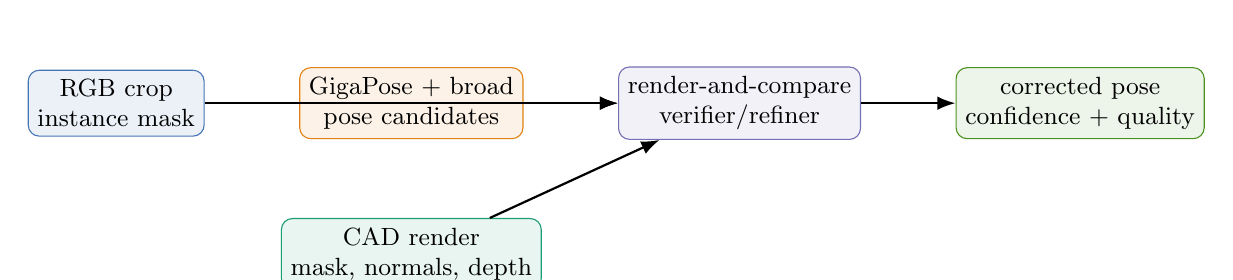
\begin{tikzpicture}[node distance=10mm and 12mm,>=Latex,font=\small]
\node[draw=rgbblue,fill=rgbblue!10,rounded corners,align=center] (obs) {RGB crop\\instance mask};
\node[draw=kalmanorange,fill=kalmanorange!10,rounded corners,align=center,right=of obs] (cand) {GigaPose + broad\\pose candidates};
\node[draw=dinoteal,fill=dinoteal!10,rounded corners,align=center,below=of cand] (cad) {CAD render\\mask, normals, depth};
\node[draw=grupurple,fill=grupurple!10,rounded corners,align=center,right=of cand] (verify) {render-and-compare\\verifier/refiner};
\node[draw=graphgreen,fill=graphgreen!10,rounded corners,align=center,right=of verify] (out) {corrected pose\\confidence + quality};
\draw[->,thick] (obs)--(verify);
\draw[->,thick] (cand)--(verify);
\draw[->,thick] (cad)--(verify);
\draw[->,thick] (verify)--(out);
\end{tikzpicture}
\caption{Frame-local RGB/mask/CAD recovery.  Rendered CAD depth is candidate geometry, not observed sensor depth.}
\end{figure}

\subsection{Result}

On the final benchmark, the CNN recovery reduced GigaPose translation mean from $9.703$ to $5.529\unitm$, but rotation became worse ($43.68\rightarrow55.52\unitdeg$).  This established the first recurring lesson: image/CAD matching could repair depth while selecting a wrong symmetric orientation.

\section{Visual backbone progression: CNN, DINO, and U-Net matching}

\subsection{Architectures tested}

The visual experiments preserved the same candidate-search and pose heads while changing the evidence encoder.
\begin{enumerate}
\item \textbf{CNN baseline}: the original RGB/mask branch and CAD branch.
\item \textbf{Frozen pooled DINO}: frozen DINOv2-S/14 evidence projected into the CNN/CAD representation.
\item \textbf{DINO last-block tuning}: only DINO's final transformer block was unfrozen.
\item \textbf{Matching U-Net}: observed and rendered feature pyramids were fused with concatenation, absolute difference, and product; a decoder retained spatial correspondence.
\item \textbf{Frozen-DINO matching U-Net}: a $16\times16$ DINO patch map was fused into the matching decoder rather than immediately pooled.
\item \textbf{DINO matching U-Net last block}: the final DINO block was additionally tuned.
\end{enumerate}

For matching features $F_o,F_c$, the core fusion is schematically
\begin{equation}
F_{\rm match}=\operatorname{UNet}\bigl([F_o,F_c,|F_o-F_c|,F_o\odot F_c]\bigr).
\end{equation}
The frozen-DINO matching U-Net has about $3.19$ million trainable non-DINO parameters and computes observed-image DINO features once per frame, reusing them across all CAD candidates.

\subsection{Preliminary seven-backbone development comparison}

Table~\ref{tab:devbackbones} reports the ungated Putnam-rear development sequence.  These numbers guided architecture selection; they are not the 5,174-frame final benchmark.  Translation improved for DINO last-block and DINO matching variants, while rotation instability remained severe.  Frozen DINO alone did not guarantee improvement, and unfreezing DINO could overfit orientation.

\begin{table}[H]
\centering
\caption{Putnam-rear development comparison (mean errors; preliminary).}
\label{tab:devbackbones}
\begin{tabular}{lrr}
\toprule
Model & Translation (m) & Rotation (deg)\\
\midrule
GigaPose & 9.812 & 76.01\\
CNN multi-checkpoint & 6.707 & 80.98\\
Frozen pooled DINO & 10.367 & 121.06\\
DINO final block tuned & 5.426 & 78.98\\
Matching U-Net & 7.544 & 77.09\\
Frozen-DINO matching U-Net & 5.451 & 83.03\\
DINO matching U-Net, final block tuned & \best{4.248} & 122.76\\
\bottomrule
\end{tabular}
\end{table}

\subsection{Final benchmark: CNN versus frozen-DINO matching U-Net}

Only CNN and frozen-DINO matching U-Net were carried into the final benchmark suite.  DINO matching improved translation mean/RMSE from $5.529/10.001$ to $4.460/7.934\unitm$ and rotation mean from $55.52$ to $40.47\unitdeg$.  It beat the CNN in translation from 20--140 m and was especially useful at long range, but neither per-frame verifier solved temporal orientation reliably.

\begin{table}[H]
\centering
\caption{Final benchmark frame-local visual recovery.}
\begin{tabular}{lrrrrrr}
\toprule
Model & $t$ mean & $t$ RMSE & $R$ mean & $R$ RMSE & ADD mean & ADD RMSE\\
\midrule
GigaPose & 9.703 & 16.914 & 43.68 & 71.18 & 9.805 & 16.942\\
CNN recovery & 5.529 & 10.001 & 55.52 & 90.20 & 5.803 & 10.046\\
DINO matching U-Net recovery & \best{4.460} & \best{7.934} & \best{40.47} & \best{76.03} & \best{4.621} & \best{7.967}\\
\bottomrule
\end{tabular}
\end{table}

\begin{table}[H]
\centering
\caption{Translation mean by distance for frame-local recovery (m).}
\begin{tabular}{lrrrrrrr}
\toprule
Model & 0--20 & 20--40 & 40--60 & 60--80 & 80--100 & 100--120 & 120--140\\
\midrule
GigaPose & 1.830 & 5.087 & 7.715 & 9.638 & 16.926 & 26.206 & 30.868\\
CNN & \best{0.930} & 2.277 & 4.576 & 7.439 & 12.278 & 13.492 & 14.999\\
DINO matching U-Net & 1.199 & \best{2.101} & \best{3.485} & \best{6.556} & \best{9.870} & \best{9.153} & \best{11.138}\\
\bottomrule
\end{tabular}
\end{table}

\section{Temporal candidate selection with a GRU}

\subsection{From a deterministic window to a learned selector}

The first no-retraining temporal extension used a five-frame candidate path.  For candidate sequence $c_{t-W+1:t}$,
\begin{equation}
E=\lambda_u\sum_k E_{\rm RGB}(c_k)+E_{\rm speed}+E_{\rm acceleration}+E_{\rm rotation}+E_{\rm angular\ acceleration},\qquad W=5.
\end{equation}
With four retained candidates per frame, exhaustive selection examines at most $4^5=1024$ paths.  This was replaced by an eight-frame causal GRU that scores 16 candidates per frame.  For logits $a_{t,i}$,
\begin{equation}
p(c_t=i\mid\mathcal H_t)=\operatorname{softmax}_i(a_{t,i}),\qquad
\mathcal L_{\rm select}=-\sum_t\log p(c_t=c_t^*\mid\mathcal H_t).
\end{equation}
Candidate zero is always untouched GigaPose, giving an explicit fallback.  Sequence state resets at run, camera, frame-gap, or timestamp discontinuities.

\subsection{Orientation hysteresis and fixed lag}

The selector's temporal-orientation layer compares candidates with previous orientation, angular-velocity prediction, and an explicit opposite-mode hypothesis.  Soft penalties start near $45\unitdeg$; candidates beyond $90\unitdeg$ are held; a mode change beyond $135\unitdeg$ requires repeated confirmation.  Fixed lag buffers pending rows and backfills the start of a confirmed transition.  On the Laguna/Putnam validation experiment, temporal orientation changed rotation mean from $20.60$ to $16.91\unitdeg$ while translation remained approximately $2.57\unitm$.

\subsection{Final benchmark result}

The GRU selector plus fixed-lag orientation reduced frame-local DINO recovery from $4.460$ to $3.626\unitm$ translation mean and from $40.47$ to $14.11\unitdeg$ rotation mean.  It selected a recovery candidate on $98.6\%$ of frames, temporally reranked 51 frames, used orientation fallback on 232 frames, confirmed 29 flip transitions, and backfilled 59 rows.

\section{GRU--Kalman filtering and cascade ordering}

\subsection{Learned SE(3) filtering}

The GRU--Kalman state contains pose and learned motion,
\begin{equation}
\bm x_t=(\bm p_t,R_t,\bm v_t,\bm\omega_t).
\end{equation}
A simplified prediction is
\begin{align}
\bm p^-_t&=\bm p_{t-1}+\Delta t\,\bm v_{t-1},\\
R^-_t&=R_{t-1}\operatorname{Exp}(\Delta t\,\bm\omega_{t-1}),
\end{align}
with translation and rotation innovations
\begin{align}
\bm r^p_t&=\bm z^p_t-\bm p^-_t,\\
\bm r^R_t&=\log\bigl((R^-_t)^TR^z_t\bigr).
\end{align}
A causal GRU predicts diagonal gains $K^p_t,K^R_t$ and updates
\begin{align}
\bm p_t&=\bm p^-_t+K^p_t\odot\bm r^p_t,\\
R_t&=R^-_t\operatorname{Exp}(K^R_t\odot\bm r^R_t).
\end{align}

\subsection{Alone versus selector prior}

Filtering raw GigaPose alone was weak: translation mean improved only $9.703\rightarrow9.100\unitm$ and rotation $43.68\rightarrow43.36\unitdeg$, with a 41.3\% fallback rate.  The measurement distribution was too poor and multimodal for local filtering.

Using the GRU selector as the measurement/prior changed the outcome.  A newly trained translation-only filter reduced selector translation from $3.626$ to $2.423\unitm$ while preserving selector orientation at $14.11\unitdeg$.  A full-pose filter reached $2.720\unitm$ and $12.75\unitdeg$.  Therefore translation-only filtering gave the stronger balanced result; full-pose filtering traded translation for modest rotation improvement.

\begin{table}[H]
\centering
\caption{Final benchmark: modules alone and in cascade.}
\begin{tabular}{lrrrrrr}
\toprule
System & $t$ mean & $t$ RMSE & $R$ mean & $R$ RMSE & ADD mean & ADD RMSE\\
\midrule
GigaPose & 9.703 & 16.914 & 43.68 & 71.18 & 9.805 & 16.942\\
RGB recovery (CNN) & 5.529 & 10.001 & 55.52 & 90.20 & 5.803 & 10.046\\
DINO recovery & 4.460 & 7.934 & 40.47 & 76.03 & 4.621 & 7.967\\
GRU selector + orientation lag & 3.626 & 8.263 & 14.11 & 33.01 & 3.673 & 8.282\\
GRU--Kalman alone & 9.100 & 16.763 & 43.36 & 70.37 & 9.249 & 16.816\\
Selector $\rightarrow$ translation filter & \best{2.423} & \best{4.406} & 14.11 & 33.01 & \best{2.470} & \best{4.429}\\
Selector $\rightarrow$ full-pose filter & 2.720 & 5.796 & \best{12.75} & \best{32.20} & 2.761 & 5.814\\
\bottomrule
\end{tabular}
\end{table}

\subsection{Learned component fallback heads}

Translation- and rotation-trust heads were trained to estimate whether a refined component beat GigaPose:
\begin{equation}
y^t=\mathbb 1[e^t_{\rm refined}+m_t<e^t_{\rm GP}],\qquad
y^R=\mathbb 1[e^R_{\rm refined}+m_R<e^R_{\rm GP}].
\end{equation}
Held-out-head variants did not improve the benchmark: the final fallback system produced $5.016\unitm$ and $19.37\unitdeg$, substantially worse than the unchanged full cascade.  These heads were therefore disabled in later primary comparisons.  This negative result motivated deterministic sequence-consistency repair rather than a frame-local learned fallback decision.

\section{Fixed-lag translation and orientation repair}

\subsection{Translation repair}

The fixed-lag translation stage receives the causal GRU--Kalman trajectory and candidate translations from the selector, RGB recovery, and GigaPose.  In a local lag window it predicts a motion-consistent location $\tilde{\bm p}_t$ and evaluates candidate residuals, schematically
\begin{equation}
E_i=\lambda_p\|\bm p_{t,i}-\tilde{\bm p}_t\|_{\rho}^2+
\lambda_v\|\bm v_{t,i}-\tilde{\bm v}_t\|_{\rho}^2+
\lambda_a\|\bm a_{t,i}\|_{\rho}^2.
\end{equation}
An alternate candidate must improve the trajectory residual by a configured margin; rotation is copied from the causal output.  On the benchmark it repaired 123 frames (2.38\%), selected GigaPose translation 103 times and selector translation 20 times, and improved 73.2\% of repaired frames.

\paragraph{What state replay means.}
The direct fixed-lag stage changes the reported translation at a repaired frame, but it does \emph{not} retroactively change the GRU hidden state that was computed from the original measurement.  Consequently, later causal states still carry information from the rejected translation.  Replay tests whether feeding the repaired measurements back through the same trained GRU--Kalman model improves that downstream state.  If $\bm z_t$ is the original selector measurement, $\bm z'_t$ is its fixed-lag-corrected version, and $F_\theta$ is the recurrent filter, the first pass and replay are
\begin{equation}
(\bm h_t,\hat T_t)=F_\theta(\bm h_{t-1},\bm z_t),\qquad
(\bm h'_t,\hat T'_t)=F_\theta(\bm h'_{t-1},\bm z'_t).
\end{equation}
The implementation reruns each complete contiguous segment with the corrected measurement sequence.  This is equivalent to restoring the recurrent state before the earliest repair and processing forward, while avoiding a change to the existing GRU API.  It is still inference-only: no ground truth or retraining is used.

Two outputs isolate the effect of recurrent-state propagation.  \emph{Translation-only replay}, the recommended variant, takes the replayed translation but preserves the original causal rotation,
\begin{equation}
T_t^{\mathrm{replay},t}=\begin{bmatrix}R_t^{\mathrm{causal}}&\bm t'_t\\\bm 0^\top&1\end{bmatrix}.
\end{equation}
\emph{Full-pose replay} is diagnostic and accepts both replayed components,
$T_t^{\mathrm{replay},SE(3)}=\hat T'_t$, so a translation repair may also alter subsequent rotation through the shared recurrent state.

\begin{table}[H]
\centering
\caption{Fixed-lag and replay ablation on 5,174 frames.}
\begin{tabular}{lrrrrr}
\toprule
System & $t$ mean & $t$ RMSE & $t$ median & $t$ P90 & $R$ mean\\
\midrule
Causal GRU--Kalman & 2.491 & 4.316 & 1.120 & 6.702 & 12.04\\
Fixed-lag translation & \best{2.454} & \best{4.255} & 1.114 & 6.615 & 12.04\\
Replay, translation only & 2.460 & 4.263 & \best{1.111} & \best{6.606} & 12.04\\
Replay, full pose & 2.460 & 4.263 & \best{1.111} & \best{6.606} & \best{12.03}\\
\bottomrule
\end{tabular}
\end{table}

Fixed-lag repair produced a real but small gain: $0.037\unitm$ in mean translation and $0.061\unitm$ in RMSE.  Replay slightly improved median and P90 but not mean or RMSE relative to the direct repair, indicating that recurrent propagation sometimes moved later estimates away from otherwise-good causal outputs.  Translation-only and full-pose replay have identical translation by construction; full-pose replay changed orientation and improved rotation mean only marginally ($12.04\unitdeg\rightarrow12.03\unitdeg$).

\section{Lag-masked candidate transformers}

\subsection{Numeric and frozen-visual designs}

Both transformers use an eight-frame window, 16 candidates per frame, model width 128, four heads, two temporal cross-attention layers, and future lag $\ell=4$.  The lag-aware mask is
\begin{equation}
M_{ij}=\begin{cases}0,&j\le i+\ell,\\-\infty,&j>i+\ell.\end{cases}
\end{equation}
Thus the deployed fixed-lag target sees its permitted future context while earlier queries cannot leak arbitrarily far future evidence.

\paragraph{Why this model size was chosen.}
These values were conservative engineering defaults for the first controlled transformer experiment, not the result of a complete architecture sweep.  The training set contains 9,795 frames but only 15 independent physical runs, so increasing capacity aggressively would add overfitting risk; indeed, the visual model selected its best-pose checkpoint at epoch 4.  The individual choices were:

\begin{itemize}
\item \textbf{Eight frames with lag four.}  For the deployed target at index $8-4-1=3$, the window supplies three past frames, the current frame, and four permitted future frames.  This is long enough to estimate velocity, acceleration, and jerk and to resolve a short orientation/depth ambiguity, while limiting latency to four frames.  A longer window would increase latency and reduce the number of independent training windows.
\item \textbf{Sixteen candidates per frame.}  This number is determined upstream by the candidate-export budget: candidate zero is the original rank-0 GigaPose pose and up to 15 highest-ranked RGB/CAD recovery hypotheses are retained from a pool of at most 48.  It preserves multiple yaw, flip, depth, center, and rotation alternatives without passing every weak proposal downstream.  Thus each temporal sample contains $8\times16=128$ candidate poses.  This is a search-coverage/computation tradeoff, not a claim that candidate 17 can never be useful.
\item \textbf{Width 128 and four heads.}  A width of 128 is large enough to project the 23 numeric candidate features, eight frame features, and optional visual embeddings into a common representation while keeping the models small (697,169 numeric and 901,713 visual trainable parameters).  Four heads give 32 dimensions per head, allowing several relation subspaces without the narrow 16-dimensional heads that an eight-head version would have at the same width.
\item \textbf{Two temporal cross-attention layers.}  The first layer gathers lag-permitted frame evidence; the second can refine that representation after its feed-forward transformation.  More layers would increase capacity and optimization difficulty for a relatively small run-level dataset.  Importantly, ``two'' refers only to the main temporal stack: the model also has per-frame candidate cross-attention and a separate one-layer lag-masked translation-refinement branch.
\item \textbf{Feed-forward width 256.}  The $2\times$ expansion supplies nonlinear mixing without the $4\times$ expansion commonly used in much larger language/vision transformers, again favoring regularization and memory efficiency.
\end{itemize}

Accordingly, the present comparison answers whether numeric versus frozen-visual evidence helps under a matched, compact architecture.  It does \emph{not} establish that $(L,N,d,H,K)=(8,16,128,4,2)$ is optimal.  A proper ablation should vary one axis at a time---for example $N\in\{8,16,24\}$, $d\in\{64,128,192\}$, $H\in\{2,4,8\}$, $K\in\{1,2,3\}$, and lag/window pairs $(4,2),(8,4),(12,4)$---and select by run-held-out pose RMSE rather than training loss.

The \textbf{numeric transformer} consumes 23 candidate and eight frame features and has 697,169 trainable parameters.  The \textbf{frozen visual-fusion transformer} additionally consumes cached 384-dimensional frame vectors and 432-dimensional candidate matching vectors from the frozen DINO matching U-Net; it has 901,713 trainable parameters and does not duplicate or train DINO.  Both include a learned translation fixed-lag branch supervised by position, velocity, acceleration, and jerk:
\begin{equation}
\mathcal L_{\rm seq}=\lambda_p\mathcal L_p+\lambda_v\mathcal L_v+
\lambda_a\mathcal L_a+\lambda_j\mathcal L_j.
\end{equation}

\begin{figure}[p]
\centering
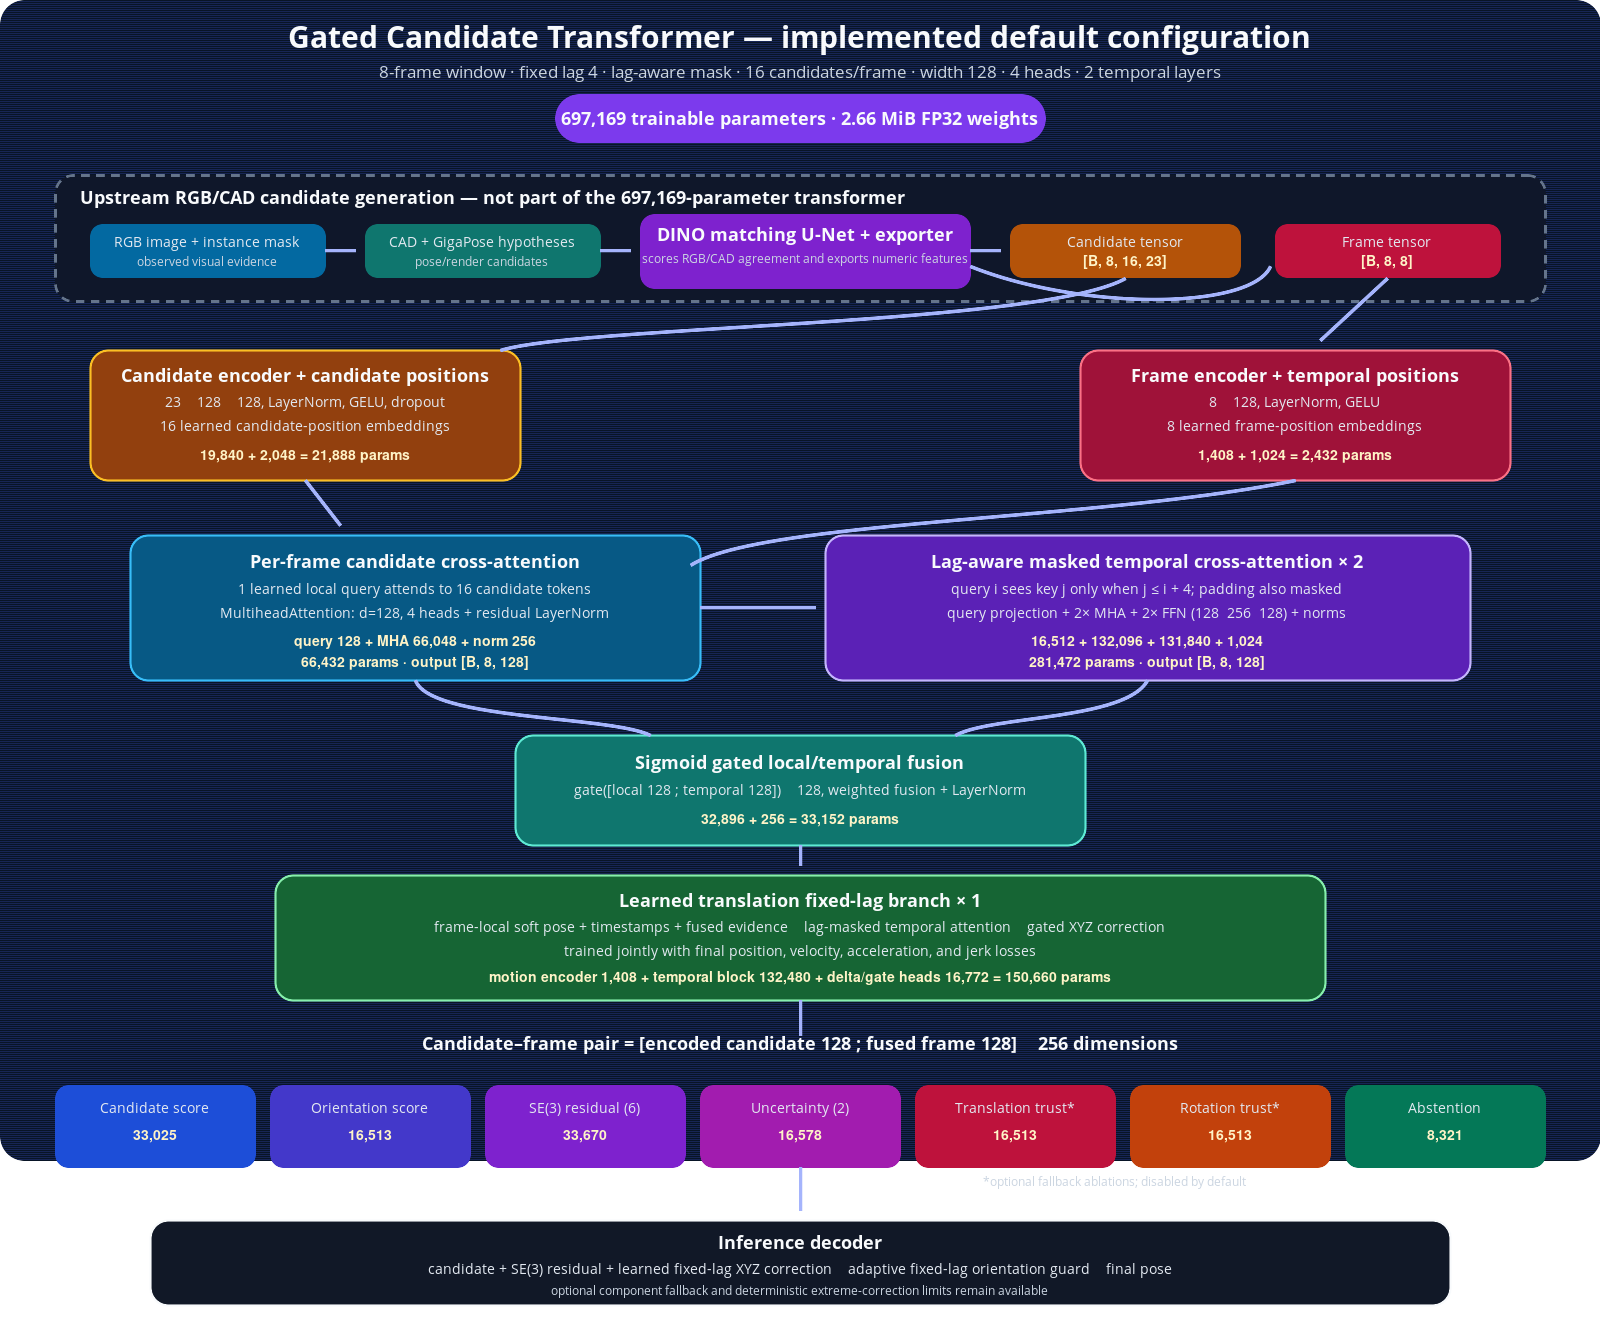
\includegraphics[width=0.96\textwidth]{../../tracking/rgb_self_recovery/sliding_window/gated_candidate_transformer/transformer_architecture.png}
\caption{Implemented candidate-transformer architecture.  Candidate cross-attention and lag-masked temporal attention feed pose, uncertainty, trust, abstention, and fixed-lag branches.}
\end{figure}

The visual model reached its best-pose checkpoint at epoch 4 and then strongly overfit: training candidate loss continued falling while validation candidate loss rose.  Early stopping preserved the useful checkpoint.  On validation, visual fusion improved numeric translation RMSE $2.613\rightarrow1.712\unitm$ and rotation mean $11.38\rightarrow8.76\unitdeg$.

\subsection{Final benchmark performance and distance crossover}

\begin{table}[H]
\centering
\caption{Transformer comparison with the strongest pre-transformer cascades.}
\begin{tabular}{lrrrrrr}
\toprule
System & $t$ mean & $t$ RMSE & $R$ mean & $R$ RMSE & ADD mean & ADD RMSE\\
\midrule
Translation cascade & 2.423 & 4.406 & 14.11 & 33.01 & 2.470 & 4.429\\
Full-pose cascade & 2.720 & 5.796 & 12.75 & 32.20 & 2.761 & 5.814\\
Numeric transformer & 3.994 & 9.704 & 13.44 & 31.83 & 4.033 & 9.724\\
Frozen visual transformer & 3.508 & 9.544 & \best{10.83} & \best{27.48} & 3.538 & 9.560\\
\bottomrule
\end{tabular}
\end{table}

The visual transformer improves the numeric transformer and gives the strongest completed overall rotation.  Its translation mean is worse than the cascades because a minority of long-range failures dominate RMSE.  Translation-within-$1\unitm$ recall is nevertheless highest for the visual transformer (54.8\%), showing that it improves many ordinary frames while producing catastrophic tails.

\begin{table}[H]
\centering
\caption{Mean translation error by distance: frozen visual transformer versus translation cascade (m).}
\begin{tabular}{lrrrrrrr}
\toprule
Model & 0--20 & 20--40 & 40--60 & 60--80 & 80--100 & 100--120 & 120--140\\
\midrule
Visual transformer & \best{0.409} & \best{0.805} & \best{1.840} & 4.651 & 7.021 & 9.744 & 16.979\\
Translation cascade & 0.682 & 0.980 & 2.092 & \best{3.979} & \best{4.910} & \best{5.273} & \best{6.264}\\
\bottomrule
\end{tabular}
\end{table}

The crossover occurs near 60 m.  Direct visual evidence is highly valuable while the car crop still contains enough discriminative structure; at long range the visual model can commit to a wrong depth/candidate basin.

\clearpage
\section{Complete-sequence SciPy factor graph}

\subsection{Objective and modes}

For one contiguous sequence with poses $X_{1:T}$ and selected candidate measurements $Z_{t,c_t}$, the batch objective is
\begin{align}
E(X,c)=&\sum_t \rho\!\left(\|\log(Z_{t,c_t}^{-1}X_t)\|_{\Sigma_z}^2\right)
+\sum_t\rho\!\left(\|\log(P_t^{-1}X_t)\|_{\Sigma_p}^2\right)\\
&+\sum_t\rho\!\left(\|\bm a_t\|_{\Sigma_a}^2\right)
+\sum_t\rho\!\left(\|\bm\alpha_t\|_{\Sigma_\alpha}^2\right)
+\sum_t\rho\!\left(\|\bm j_t\|_{\Sigma_j}^2\right).
\end{align}
The optional $P_t$ is a cascade or transformer prior.  Candidate assignment alternates with sparse nonlinear least squares; assignment combines RGB/CAD cost, distance from the current pose, and bidirectional neighbor interpolation.

Mode A used candidates only.  Mode B added a soft external trajectory prior.  The graph sees the complete sequence, so no fixed-lag post-filter is needed for offline operation.

\subsection{Prior ablation}

\begin{table}[H]
\centering
\caption{SciPy factor-graph benchmark.}
\begin{tabular}{lrrrrrr}
\toprule
System & $t$ mean & $t$ RMSE & $R$ mean & $R$ RMSE & ADD mean & ADD RMSE\\
\midrule
Candidates-only graph & 5.454 & 10.920 & 52.37 & 83.13 & 5.713 & 10.979\\
Full-cascade prior + graph & 2.528 & 4.819 & 12.01 & 30.02 & 2.564 & 4.837\\
Translation-cascade prior + graph & \best{2.240} & \best{3.674} & \best{11.45} & \best{29.76} & \best{2.276} & \best{3.695}\\
\bottomrule
\end{tabular}
\end{table}

Candidates alone were insufficient: hard assignment changed 3,544 candidates and often selected symmetric/wrong-depth trajectories.  A strong external prior kept the nonlinear graph in the correct basin.  The translation cascade was the best prior, improving both its own translation and orientation.

\begin{table}[H]
\centering
\caption{Best completed model: translation-cascade-prior SciPy graph, by distance.}
\begin{tabular}{lrrrrrrr}
\toprule
Distance (m) & 0--20 & 20--40 & 40--60 & 60--80 & 80--100 & 100--120 & 120--140\\
\midrule
$t$ mean (m) & 0.683 & 0.920 & 1.896 & 3.674 & 4.567 & 4.907 & 5.538\\
$R$ mean (deg) & 11.41 & 5.85 & 7.65 & 19.98 & 21.28 & 11.86 & 23.05\\
ADD mean (m) & 0.765 & 0.936 & 1.911 & 3.711 & 4.605 & 4.956 & 5.606\\
\bottomrule
\end{tabular}
\end{table}

\section{GTSAM sequence optimization}

\subsection{Implementation differences}

GTSAM represents translation as \texttt{Point3} and orientation as \texttt{Rot3}, with native manifold retraction and Levenberg--Marquardt optimization.  Candidate and prior factors use built-in priors; translation acceleration/jerk and SO(3) angular acceleration use custom factors.  The formulation is close to the SciPy graph but not identical: SciPy has bounded six-dimensional increments and scalar robust residuals, while GTSAM uses factor-vector robustification and post-solve safety rejection.

The speed difference was large: the five-outer-iteration SciPy translation-prior run took $5772$ s, versus about $82$ s for GTSAM---approximately $70\times$ faster.  GTSAM rejected six of 68 translation-prior segments because proposed updates exceeded the $20\unitm$ safety limit; the full-pose-prior run rejected 15 segments.

\subsection{Prior and component ablations}

\begin{table}[H]
\centering
\caption{GTSAM prior comparison.}
\begin{tabular}{lrrrrrr}
\toprule
Prior source / components & $t$ mean & $t$ RMSE & $R$ mean & $R$ RMSE & ADD mean & ADD RMSE\\
\midrule
Translation cascade / translation only & 2.416 & 4.183 & 12.28 & 29.62 & 2.448 & 4.200\\
Full-pose cascade / full & 2.683 & 5.591 & \best{11.85} & 29.59 & 2.716 & 5.610\\
Translation cascade / full & \best{2.409} & \best{4.174} & 11.94 & \best{29.44} & \best{2.441} & \best{4.190}\\
\bottomrule
\end{tabular}
\end{table}

Using the translation cascade but retaining its rotation as a soft prior produced the strongest balanced GTSAM result.  Relative to the original translation cascade, it improved translation RMSE $4.406\rightarrow4.174\unitm$ and rotation mean $14.11\rightarrow11.94\unitdeg$.  However, translation median worsened $1.090\rightarrow1.214\unitm$ and within-$1\unitm$ recall fell from 47.0\% to 41.7\%: GTSAM reduced large tails while moving many already-good frames slightly.

The current improvement path is to use non-robust safety priors, robust candidate factors, staged continuation from strong to weaker priors, confidence-adaptive factor noise, and per-frame/interval repair instead of rejecting an entire segment.  For moving real cameras, optimization should occur in a world frame via
\begin{equation}
T_{\rm world,object}=T_{\rm world,camera}T_{\rm camera,object}.
\end{equation}

\section{Best completed results and qualitative examples}

No single model dominates every criterion.  The visual-transformer-prior SciPy graph has the best completed rotation and the best 20--80 m translation; the unmodified visual transformer remains best at 0--20 m.  The translation-cascade-prior SciPy graph has the best completed overall translation, translation RMSE, ADD, and long-range robustness.  It is therefore the current best balanced model on this development benchmark.

\begin{table}[H]
\centering
\caption{Current leaders.}
\begin{tabular}{lll}
\toprule
Criterion & Best completed system & Result\\
\midrule
Overall translation mean/RMSE & Translation prior + SciPy graph & $2.240/3.674\unitm$\\
Overall ADD mean/RMSE & Translation prior + SciPy graph & $2.276/3.695\unitm$\\
Overall rotation mean/RMSE & Visual prior + SciPy graph & $9.26/24.68\unitdeg$\\
0--20 m translation mean & Frozen visual transformer & $0.409\unitm$\\
20--40 m translation mean & Visual prior + SciPy graph & $0.685\unitm$\\
40--60 m translation mean & Visual prior + SciPy graph & $1.275\unitm$\\
60--80 m translation mean & Visual prior + SciPy graph & $3.160\unitm$\\
120--140 m translation mean & Translation prior + SciPy graph & $5.538\unitm$\\
Fast batch optimizer & Translation/full-components GTSAM & $\sim82$ s\\
\bottomrule
\end{tabular}
\end{table}

\begin{figure}[H]
\centering
\includegraphics[width=0.98\textwidth]{../../gigaPose_datasets/results/transformer_visual_fusion_test/all_models_comparison/overlays/000001_000219_depth86.0m.jpg}
\caption{A frame where direct visual fusion is decisive.  At 86 m the frozen visual transformer has $0.94\unitm$ translation error, while the translation-prior graph is trapped at $20.37\unitm$.  This demonstrates why visual evidence should not be discarded.}
\end{figure}

\begin{figure}[H]
\centering
\includegraphics[width=0.98\textwidth]{../../gigaPose_datasets/results/transformer_visual_fusion_test/all_models_comparison/overlays/000001_000975_depth125.3m.jpg}
\caption{A catastrophic visual-transformer long-range failure.  At 125.3 m, GigaPose and both transformers remain near $50.87\unitm$ translation error, whereas the translation-cascade-prior graph reaches $2.10\unitm$.}
\end{figure}

\begin{figure}[H]
\centering
\includegraphics[width=0.98\textwidth]{../../gigaPose_datasets/results/transformer_visual_fusion_test/all_models_comparison/overlays/000001_000199_depth113.4m.jpg}
\caption{A difficult 113.4 m frame where several refiners repair a $77.44\unitm$ GigaPose failure.  Numeric and visual transformers are below $1\unitm$; the translation-prior graph reaches $1.54\unitm$.}
\end{figure}

\begin{figure}[H]
\centering
\begin{subfigure}{0.32\textwidth}
\includegraphics[width=\textwidth]{../../gigaPose_datasets/results/transformer_visual_fusion_test/all_models_comparison/translation_error_by_distance.png}
\caption{Translation}
\end{subfigure}\hfill
\begin{subfigure}{0.32\textwidth}
\includegraphics[width=\textwidth]{../../gigaPose_datasets/results/transformer_visual_fusion_test/all_models_comparison/rotation_error_by_distance.png}
\caption{Rotation}
\end{subfigure}\hfill
\begin{subfigure}{0.32\textwidth}
\includegraphics[width=\textwidth]{../../gigaPose_datasets/results/transformer_visual_fusion_test/all_models_comparison/add_by_distance.png}
\caption{ADD}
\end{subfigure}
\caption{Distance-binned comparison before adding GTSAM.  The visual transformer leads at short range; the translation-cascade graph is much more stable at long range.}
\end{figure}

\section{Visual transformer as a graph prior}

This experiment tested whether complete-sequence optimization could retain the visual transformer's strong short/mid-range accuracy and orientation while suppressing its long-range translation outliers.  It used the \emph{exact transformer test candidate bundle}; those candidates differ from the older cascade-graph export even though frame keys and ground truth match.  Comparisons with older prior runs therefore compare complete systems, not only the prior in isolation.

\begin{table}[H]
\centering
\caption{Frozen-visual-transformer prior experiment on 5,174 frames.}
\begin{tabular}{lrrrrrr}
\toprule
System & $t$ mean & $t$ RMSE & $R$ mean & $R$ RMSE & ADD mean & ADD RMSE\\
\midrule
Frozen visual transformer & 3.508 & 9.544 & 10.83 & 27.48 & 3.538 & 9.560\\
Visual $\rightarrow$ SciPy graph & \best{2.697} & \best{6.920} & \best{9.26} & \best{24.68} & \best{2.717} & \best{6.933}\\
Visual $\rightarrow$ GTSAM full prior & 3.587 & 9.510 & 10.75 & 26.92 & 3.610 & 9.527\\
Visual $\rightarrow$ GTSAM translation prior & 3.588 & 9.511 & 11.19 & 27.14 & 3.611 & 9.528\\
\bottomrule
\end{tabular}
\end{table}

The SciPy graph clearly succeeded: relative to the visual transformer it reduced translation mean by $0.812\unitm$, translation RMSE by $2.624\unitm$, rotation mean by $1.58\unitdeg$, and rotation RMSE by $2.80\unitdeg$.  It improved translation on 53.7\% of paired frames and rotation on 59.2\%; both components improved together on 34.9\%.  Its only distance-bin translation regression was 0--20 m ($0.409\rightarrow0.478\unitm$).  Mean translation improved at 20--40, 40--60, 60--80, 80--100, 100--120, and 120--140 m from $0.805,1.840,4.651,7.021,9.744,16.979\unitm$ to $0.685,1.275,3.160,5.069,7.485,13.853\unitm$, respectively.

The visual-prior GTSAM variants were conservative but unsuccessful overall.  Both accepted only 33 of 68 segments (48.5\%); rejected segments retained the original visual prediction.  Full-prior GTSAM improved rotation slightly but worsened translation mean $3.508\rightarrow3.587\unitm$, and translation-only-prior GTSAM also worsened rotation.  The 120--140 m outputs were unchanged, so GTSAM did not repair the visual model's most important long-range tail.

Compared with previous priors, visual+SciPy now dominates translation-cascade+SciPy through 60--80 m and dominates every previous system in overall rotation.  The translation-cascade+SciPy graph remains superior at 80--100 m ($4.567$ versus $5.069\unitm$), 100--120 m ($4.907$ versus $7.485\unitm$), and 120--140 m ($5.538$ versus $13.853\unitm$), yielding the better overall translation mean/RMSE ($2.240/3.674$ versus $2.697/6.920\unitm$).  This confirms that the useful next design is confidence- or distance-adaptive prior fusion rather than choosing one fixed prior globally.

\section{Conclusions}

\begin{enumerate}
\item Frame-local RGB/CAD recovery materially reduced GigaPose translation but could worsen front/rear orientation.
\item Frozen DINO spatial matching was more useful than pooled frozen DINO alone; visual pretraining did not automatically improve pose without correspondence structure.
\item Temporal candidate selection was essential for orientation and reduced DINO recovery translation further.
\item A GRU--Kalman model was ineffective on raw GigaPose but effective after the selector changed the measurement distribution.
\item Translation-only cascade filtering produced the strongest recurrent cascade; full-pose filtering traded translation for rotation.
\item Fixed-lag translation repair improved only 123 frames but reduced mean/RMSE without using ground truth at inference.
\item The visual transformer strongly improved near/mid-range and rotation; using it as a SciPy prior improved it further and produced the best rotation result, but long-range translation remained weaker than the translation-cascade-prior graph.
\item A candidates-only batch factor graph failed.  Priors were necessary to resolve candidate ambiguity.
\item The translation-cascade-prior SciPy graph is the strongest completed balanced system.
\item GTSAM retained most of the benefit at about $70\times$ lower optimization time, but its current safety/prior formulation is less accurate in translation.
\item The next model experiment is confidence- or distance-adaptive fusion of visual and cascade priors; the next evaluation requirement is a genuinely untouched physical run.
\end{enumerate}

\appendix
\small
\section{Result provenance}

Primary machine-readable sources used in this report:
\begin{itemize}
\item \texttt{.../comparison/full\_benchmark/summary.json}: RGB recovery, GRU, Kalman, and cascades.
\item \texttt{.../comparison/all\_existing\_plus\_fixed\_lag\_replay/summary.json}: fixed-lag and replay.
\item \texttt{.../transformer\_visual\_fusion\_test/all\_models\_comparison/summary.json}: transformers and SciPy graph.
\item \texttt{.../transformer\_visual\_fusion\_test/frozen\_visual\_plus\_graph/comparison/summary.json}: visual-prior SciPy/GTSAM comparison.
\item \texttt{.../sequence\_factor\_graph/comparison/summary.json}: factor-graph modes.
\item \texttt{.../sequence\_factor\_graph\_gtsam/comparison\_full\_components/summary.json}: GTSAM prior components.
\item Individual \texttt{run\_report.json} files: repair counts, acceptance, timing, checkpoints, and configuration.
\end{itemize}

All paths are rooted at
\begin{quote}
\path{gigaPose_datasets/results/rgb_self_recovery_benchmark_pose_regenerated_20260803}
\end{quote}
except transformer outputs, which are rooted at
\begin{quote}
\path{gigaPose_datasets/results/transformer_visual_fusion_test}.
\end{quote}

\section{Reproducibility status}

The source packages are isolated under
\path{tracking/rgb_self_recovery/sliding_window/} and include README run commands for the GRU selector, GRU--Kalman filter, fixed-lag translation, numeric transformer, frozen visual-fusion transformer, SciPy factor graph, and GTSAM factor graph.  The GTSAM package pins \texttt{gtsam==4.2} with NumPy $<2$ and includes focused synthetic tests.  Ground truth is used by training-label generation and evaluation, but not by candidate selection, filtering, fixed-lag repair, transformer inference, or factor-graph optimization.

\section{All-model distance-binned benchmark tables}
All entries below are arithmetic means on the same 5,174-frame regenerated-pose development benchmark.  The visual-transformer graph uses its own exported candidate bundle, so comparisons with older cascade-graph runs are complete-system comparisons rather than a pure prior ablation.  Standard ADD is the mean corresponding CAD-vertex displacement produced jointly by translation and rotation.  A ``translation-only ADD'' obtained by holding rotation at ground truth is exactly the Euclidean translation error already reported; a separate rotation-only ADD was not emitted by the existing evaluator and is therefore not mislabeled here.

\begin{landscape}
\begin{table}[H]
\centering
\scriptsize
\setlength{\tabcolsep}{3.2pt}
\caption{Mean translation error by distance (m); 5,174 frames.}
\resizebox{\linewidth}{!}{\begin{tabular}{lrrrrrrrr}
\toprule
Model & Overall & 0--20 & 20--40 & 40--60 & 60--80 & 80--100 & 100--120 & 120--140\\
\midrule
GigaPose & 9.703 & 1.830 & 5.087 & 7.715 & 9.638 & 16.926 & 26.206 & 30.868\\
CNN RGB recovery & 5.529 & 0.930 & 2.277 & 4.576 & 7.439 & 12.278 & 13.492 & 14.999\\
DINO matching recovery & 4.460 & 1.199 & 2.101 & 3.485 & 6.556 & 9.870 & 9.153 & 11.138\\
GRU selector + orientation lag & 3.626 & 0.735 & 1.132 & 2.425 & 4.886 & 6.831 & 9.485 & 14.833\\
GRU--Kalman alone & 9.100 & 1.142 & 3.988 & 7.114 & 9.630 & 16.792 & 26.219 & 30.924\\
Translation cascade & 2.423 & 0.682 & 0.980 & 2.092 & 3.979 & 4.910 & 5.273 & 6.264\\
Full-pose cascade & 2.720 & 0.676 & 0.990 & 2.144 & 4.177 & 5.387 & 6.482 & 8.493\\
Fallback-head cascade (failed) & 5.016 & 1.062 & 1.537 & 4.391 & 4.592 & 5.187 & 5.536 & 6.523\\
Causal GRU--Kalman first pass & 2.491 & 0.675 & 0.992 & 2.143 & 4.158 & 5.137 & 5.536 & 6.183\\
Fixed-lag translation & 2.454 & 0.671 & 0.972 & 2.111 & 4.100 & 5.016 & 5.428 & 6.226\\
Replay: translation only & 2.460 & 0.669 & 0.968 & 2.103 & 4.128 & 4.970 & 5.505 & 6.326\\
Replay: full pose & 2.460 & 0.669 & 0.968 & 2.103 & 4.128 & 4.970 & 5.505 & 6.326\\
Numeric transformer & 3.994 & 0.503 & 1.038 & 2.366 & 5.383 & 8.322 & 10.363 & 17.948\\
Frozen visual transformer & 3.508 & \best{0.409} & 0.805 & 1.840 & 4.651 & 7.021 & 9.744 & 16.979\\
Candidates-only SciPy graph & 5.454 & 1.260 & 1.755 & 3.350 & 7.330 & 9.364 & 15.122 & 22.893\\
Full-cascade + SciPy & 2.528 & 0.673 & 0.936 & 1.974 & 3.783 & 4.824 & 6.182 & 8.016\\
Translation-cascade + SciPy & \best{2.240} & 0.683 & 0.920 & 1.896 & 3.674 & \best{4.567} & \best{4.907} & \best{5.538}\\
Translation-cascade + GTSAM ($t$ prior) & 2.416 & 0.842 & 1.083 & 1.935 & 3.774 & 4.651 & 5.457 & 5.971\\
Full-cascade + GTSAM (full prior) & 2.683 & 0.838 & 1.094 & 2.005 & 4.004 & 4.895 & 6.480 & 8.278\\
Translation-cascade + GTSAM (full components) & 2.409 & 0.839 & 1.086 & 1.931 & 3.769 & 4.637 & 5.423 & 5.930\\
Visual-transformer + SciPy & 2.697 & 0.478 & \best{0.685} & \best{1.275} & \best{3.160} & 5.069 & 7.485 & 13.853\\
Visual-transformer + GTSAM full & 3.587 & 0.721 & 0.964 & 1.775 & 4.502 & 6.900 & 9.818 & 16.979\\
Visual-transformer + GTSAM translation & 3.588 & 0.718 & 0.962 & 1.783 & 4.508 & 6.902 & 9.818 & 16.979\\
\bottomrule
\end{tabular}}
\end{table}
\end{landscape}

\begin{landscape}
\begin{table}[H]
\centering
\scriptsize
\setlength{\tabcolsep}{3.2pt}
\caption{Mean rotation error by distance (degrees); 5,174 frames.}
\resizebox{\linewidth}{!}{\begin{tabular}{lrrrrrrrr}
\toprule
Model & Overall & 0--20 & 20--40 & 40--60 & 60--80 & 80--100 & 100--120 & 120--140\\
\midrule
GigaPose & 43.68 & 48.36 & 30.41 & 35.16 & 58.76 & 53.11 & 55.90 & 75.66\\
CNN RGB recovery & 55.52 & 65.33 & 58.27 & 46.66 & 80.82 & 40.87 & 33.52 & 47.91\\
DINO matching recovery & 40.47 & 49.88 & 43.45 & 28.26 & 56.59 & 29.18 & 30.06 & 33.17\\
GRU selector + orientation lag & 14.11 & 13.33 & 7.66 & 9.78 & 22.62 & 25.95 & 16.37 & 28.28\\
GRU--Kalman alone & 43.36 & 48.16 & 30.05 & 34.89 & 59.46 & 51.74 & 55.75 & 75.26\\
Translation cascade & 14.11 & 13.33 & 7.66 & 9.78 & 22.62 & 25.95 & 16.37 & 28.28\\
Full-pose cascade & 12.75 & 12.86 & 6.67 & 8.41 & 21.27 & 23.69 & 15.42 & 22.88\\
Fallback-head cascade (failed) & 19.37 & 31.97 & 16.06 & 23.91 & 18.34 & 19.41 & 15.42 & 22.88\\
Causal GRU--Kalman first pass & 12.04 & 12.25 & 6.47 & 8.52 & 20.52 & 23.61 & 14.36 & \best{15.67}\\
Fixed-lag translation & 12.04 & 12.25 & 6.47 & 8.52 & 20.52 & 23.61 & 14.36 & \best{15.67}\\
Replay: translation only & 12.04 & 12.25 & 6.47 & 8.52 & 20.52 & 23.61 & 14.36 & \best{15.67}\\
Replay: full pose & 12.03 & 12.25 & 6.48 & 8.54 & 20.49 & 23.54 & 14.21 & 15.78\\
Numeric transformer & 13.44 & 5.67 & 7.77 & 11.63 & 17.52 & 24.04 & 21.51 & 39.16\\
Frozen visual transformer & 10.83 & 5.06 & 4.78 & 6.88 & 17.31 & 22.87 & 14.37 & 37.99\\
Candidates-only SciPy graph & 52.37 & 65.14 & 53.22 & 39.54 & 65.49 & 39.19 & 43.76 & 56.74\\
Full-cascade + SciPy & 12.01 & 12.51 & 6.34 & 7.95 & 20.41 & 21.73 & 13.93 & 21.34\\
Translation-cascade + SciPy & 11.45 & 11.41 & 5.85 & 7.65 & 19.98 & 21.28 & 11.86 & 23.05\\
Translation-cascade + GTSAM ($t$ prior) & 12.28 & 11.62 & 6.29 & 8.52 & 21.35 & 23.96 & 13.36 & 22.71\\
Full-cascade + GTSAM (full prior) & 11.85 & 12.57 & 6.15 & 7.82 & 20.30 & 21.93 & 12.84 & 21.08\\
Translation-cascade + GTSAM (full components) & 11.94 & 11.90 & 6.07 & 8.34 & 20.71 & 22.74 & 12.53 & 22.10\\
Visual-transformer + SciPy & \best{9.26} & \best{4.53} & \best{4.28} & \best{5.61} & \best{14.60} & \best{19.37} & \best{9.82} & 35.43\\
Visual-transformer + GTSAM full & 10.75 & 5.61 & 5.04 & 6.04 & 16.77 & 22.19 & 14.05 & 37.99\\
Visual-transformer + GTSAM translation & 11.19 & 6.64 & 5.68 & 6.33 & 16.68 & 22.20 & 14.07 & 37.99\\
\bottomrule
\end{tabular}}
\end{table}
\end{landscape}

\begin{landscape}
\begin{table}[H]
\centering
\scriptsize
\setlength{\tabcolsep}{3.2pt}
\caption{Mean full-pose ADD by distance (m); 5,174 frames.}
\resizebox{\linewidth}{!}{\begin{tabular}{lrrrrrrrr}
\toprule
Model & Overall & 0--20 & 20--40 & 40--60 & 60--80 & 80--100 & 100--120 & 120--140\\
\midrule
GigaPose & 9.805 & 2.138 & 5.156 & 7.764 & 9.682 & 16.952 & 26.274 & 30.997\\
CNN RGB recovery & 5.803 & 1.566 & 2.630 & 4.737 & 7.595 & 12.301 & 13.524 & 14.983\\
DINO matching recovery & 4.621 & 1.595 & 2.290 & 3.568 & 6.641 & 9.900 & 9.217 & 11.121\\
GRU selector + orientation lag & 3.673 & 0.824 & 1.162 & 2.453 & 4.952 & 6.884 & 9.528 & 14.889\\
GRU--Kalman alone & 9.249 & 1.546 & 4.124 & 7.205 & 9.689 & 16.818 & 26.289 & 31.055\\
Translation cascade & 2.470 & 0.771 & 1.007 & 2.118 & 4.023 & 4.978 & 5.327 & 6.327\\
Full-pose cascade & 2.761 & 0.766 & 1.015 & 2.162 & 4.219 & 5.430 & 6.517 & 8.543\\
Fallback-head cascade (failed) & 5.066 & 1.236 & 1.614 & 4.451 & 4.643 & 5.226 & 5.581 & 6.565\\
Causal GRU--Kalman first pass & 2.528 & 0.762 & 1.014 & 2.162 & 4.194 & 5.172 & 5.573 & 6.212\\
Fixed-lag translation & 2.490 & 0.758 & 0.995 & 2.130 & 4.136 & 5.046 & 5.465 & 6.255\\
Replay: translation only & 2.497 & 0.756 & 0.991 & 2.126 & 4.161 & 4.997 & 5.545 & 6.355\\
Replay: full pose & 2.497 & 0.756 & 0.991 & 2.126 & 4.161 & 4.997 & 5.545 & 6.355\\
Numeric transformer & 4.033 & 0.527 & 1.075 & 2.417 & 5.420 & 8.352 & 10.408 & 18.035\\
Frozen visual transformer & 3.538 & \best{0.434} & 0.822 & 1.859 & 4.719 & 7.063 & 9.772 & 17.043\\
Candidates-only SciPy graph & 5.713 & 1.793 & 2.105 & 3.483 & 7.371 & 9.417 & 15.255 & 23.012\\
Full-cascade + SciPy & 2.564 & 0.764 & 0.957 & 1.988 & 3.813 & 4.845 & 6.228 & 8.064\\
Translation-cascade + SciPy & \best{2.276} & 0.765 & 0.936 & 1.911 & 3.711 & \best{4.605} & \best{4.956} & \best{5.606}\\
Translation-cascade + GTSAM ($t$ prior) & 2.448 & 0.912 & 1.099 & 1.957 & 3.818 & 4.679 & 5.486 & 6.020\\
Full-cascade + GTSAM (full prior) & 2.716 & 0.919 & 1.110 & 2.022 & 4.037 & 4.932 & 6.505 & 8.327\\
Translation-cascade + GTSAM (full components) & 2.441 & 0.915 & 1.099 & 1.952 & 3.810 & 4.663 & 5.453 & 5.974\\
Visual-transformer + SciPy & 2.717 & 0.494 & \best{0.699} & \best{1.285} & \best{3.192} & 5.088 & 7.504 & 13.932\\
Visual-transformer + GTSAM full & 3.610 & 0.733 & 0.973 & 1.789 & 4.561 & 6.941 & 9.845 & 17.043\\
Visual-transformer + GTSAM translation & 3.611 & 0.735 & 0.972 & 1.797 & 4.565 & 6.942 & 9.845 & 17.043\\
\bottomrule
\end{tabular}}
\end{table}
\end{landscape}

\begin{landscape}
\section{Focused comparison of the final seven graph-prior modes}
\renewcommand{\arraystretch}{0.82}
\setlength{\intextsep}{4pt}
\captionsetup[table]{skip=2pt}
This subset isolates the final SciPy/GTSAM experiments.  Bold values are the minimum within these seven modes for each column.

\begin{table}[H]
\centering
\scriptsize
\setlength{\tabcolsep}{3.2pt}
\caption{Final seven modes: mean translation error by distance (m).}
\resizebox{0.96\linewidth}{!}{\begin{tabular}{lrrrrrrrr}
\toprule
Model & Overall & 0--20 & 20--40 & 40--60 & 60--80 & 80--100 & 100--120 & 120--140\\
\midrule
Translation-cascade + SciPy & \best{2.240} & 0.683 & 0.920 & 1.896 & 3.674 & \best{4.567} & \best{4.907} & \best{5.538}\\
Translation-cascade + GTSAM ($t$ prior) & 2.416 & 0.842 & 1.083 & 1.935 & 3.774 & 4.651 & 5.457 & 5.971\\
Full-cascade + GTSAM (full prior) & 2.683 & 0.838 & 1.094 & 2.005 & 4.004 & 4.895 & 6.480 & 8.278\\
Translation-cascade + GTSAM (full components) & 2.409 & 0.839 & 1.086 & 1.931 & 3.769 & 4.637 & 5.423 & 5.930\\
Visual-transformer + SciPy & 2.697 & \best{0.478} & \best{0.685} & \best{1.275} & \best{3.160} & 5.069 & 7.485 & 13.853\\
Visual-transformer + GTSAM full & 3.587 & 0.721 & 0.964 & 1.775 & 4.502 & 6.900 & 9.818 & 16.979\\
Visual-transformer + GTSAM translation & 3.588 & 0.718 & 0.962 & 1.783 & 4.508 & 6.902 & 9.818 & 16.979\\
\bottomrule
\end{tabular}}
\end{table}

\begin{table}[H]
\centering
\scriptsize
\setlength{\tabcolsep}{3.2pt}
\caption{Final seven modes: mean rotation error by distance (degrees).}
\resizebox{0.96\linewidth}{!}{\begin{tabular}{lrrrrrrrr}
\toprule
Model & Overall & 0--20 & 20--40 & 40--60 & 60--80 & 80--100 & 100--120 & 120--140\\
\midrule
Translation-cascade + SciPy & 11.45 & 11.41 & 5.85 & 7.65 & 19.98 & 21.28 & 11.86 & 23.05\\
Translation-cascade + GTSAM ($t$ prior) & 12.28 & 11.62 & 6.29 & 8.52 & 21.35 & 23.96 & 13.36 & 22.71\\
Full-cascade + GTSAM (full prior) & 11.85 & 12.57 & 6.15 & 7.82 & 20.30 & 21.93 & 12.84 & \best{21.08}\\
Translation-cascade + GTSAM (full components) & 11.94 & 11.90 & 6.07 & 8.34 & 20.71 & 22.74 & 12.53 & 22.10\\
Visual-transformer + SciPy & \best{9.26} & \best{4.53} & \best{4.28} & \best{5.61} & \best{14.60} & \best{19.37} & \best{9.82} & 35.43\\
Visual-transformer + GTSAM full & 10.75 & 5.61 & 5.04 & 6.04 & 16.77 & 22.19 & 14.05 & 37.99\\
Visual-transformer + GTSAM translation & 11.19 & 6.64 & 5.68 & 6.33 & 16.68 & 22.20 & 14.07 & 37.99\\
\bottomrule
\end{tabular}}
\end{table}

\begin{table}[H]
\centering
\scriptsize
\setlength{\tabcolsep}{3.2pt}
\caption{Final seven modes: mean full-pose ADD by distance (m).}
\resizebox{0.96\linewidth}{!}{\begin{tabular}{lrrrrrrrr}
\toprule
Model & Overall & 0--20 & 20--40 & 40--60 & 60--80 & 80--100 & 100--120 & 120--140\\
\midrule
Translation-cascade + SciPy & \best{2.276} & 0.765 & 0.936 & 1.911 & 3.711 & \best{4.605} & \best{4.956} & \best{5.606}\\
Translation-cascade + GTSAM ($t$ prior) & 2.448 & 0.912 & 1.099 & 1.957 & 3.818 & 4.679 & 5.486 & 6.020\\
Full-cascade + GTSAM (full prior) & 2.716 & 0.919 & 1.110 & 2.022 & 4.037 & 4.932 & 6.505 & 8.327\\
Translation-cascade + GTSAM (full components) & 2.441 & 0.915 & 1.099 & 1.952 & 3.810 & 4.663 & 5.453 & 5.974\\
Visual-transformer + SciPy & 2.717 & \best{0.494} & \best{0.699} & \best{1.285} & \best{3.192} & 5.088 & 7.504 & 13.932\\
Visual-transformer + GTSAM full & 3.610 & 0.733 & 0.973 & 1.789 & 4.561 & 6.941 & 9.845 & 17.043\\
Visual-transformer + GTSAM translation & 3.611 & 0.735 & 0.972 & 1.797 & 4.565 & 6.942 & 9.845 & 17.043\\
\bottomrule
\end{tabular}}
\end{table}
\end{landscape}


\end{document}
